Um programa de computador é expresso por um conjunto de sentenças em alguma
linguagem de programação.\footnote{Uma sentença (\emph{statement}) pode conter uma ou várias expressões ou instruções.
Uma única instrução numa linguagem de alto nível pode representar múltiplas
instruções de máquinas.
Programas consistem de instruções e expressões.
Uma expressão é um grupo de símbolos que representa um valor.} \todo[fancyline]{Trazer o conteúdo do rodapé pra cá?}
A forma como as sentenças de uma linguagem são executadas pelo computador é
definida por um \emph{modelo de computação} \cite{roy2004}.

O código fonte de um programa consiste de uma série de instruções que expressam
uma sequência de comandos a se seguir durante a execução — esse período é
conhecido como \emph{tempo de execução}, do inglês \emph{runtime}.
Tradicionalmente, as sentenças de uma linguagem de programação denotam essa
sequência de forma explícita.
Tais linguagens são baseadas no modelo \emph{imperativo} de computação, e são
denominadas \emph{linguagens imperativas}.

\section{Linguagens de Programação}
\label{sec:org78cb0c1}
\label{sec:langs}

Linguagens de programação são mais simples que linguagens naturais, no
entanto, elas ainda podem conter uma sintaxe surpreendentemente rica, um
conjunto de abstrações, e bibliotecas auxiliares.
Esse é essencialmente o caso de linguagens usadas para resolver problemas
reais do dia-a-dia.
\textcite{roy2004} as chamam de linguagens \emph{práticas}, que são “\textelp{}
como a caixa de ferramentas de um mecânico experiente: há várias ferramentas
diferentes para finalidades diferentes e todas estão lá por uma razão.” (p.
33; tradução nossa).

Todas as linguagens de programação possuem elementos primitivos para a
descrição de dados e das transformações, ou processos, aplicados à eles —
como a adição de dois números ou a seleção de um item de uma coleção.
Essas primitivas são definidas por regras de sintaxe — a gramática — e pela
semântica — o significado.

Linguagens imperativas geralmente oferecem comandos para lidar com estado em
tempo de execução, como declaração e atribuição de variáveis, e comandos
para controlar o caminho que o programa deve seguir, como os que decidem a
ordem de execução das sentenças — na literatura essa ordem é chamada de
\emph{fluxo de controle} de um programa.

Durante sua execução o programa segue um caminho de acordo com seu \emph{estado}
interno — ou \emph{memória}, o que um programa se lembra enquanto está ‘rodando’.
Programas com estado interno, ou \emph{statefull} em inglês, são projetados para
lembrar de eventos anteriores ou de interações com o usuário.
A informação recordada é denominada o estado do programa \cite{rouse2005}.

\section{Paradigmas de Programação}
\label{sec:orgabc65ff}
Programação é uma disciplina extensa, e linguagens práticas de programação
geralmente são bastante complicadas.
Felizmente, as ideias importantes de linguagens de programação são simples
\cite{roy2009}.
Um \emph{paradigma de programação}:

\begin{citacao}
  \textelp{} é uma abordagem para a programação de um computador baseada em
  uma teoria matemática ou um conjunto coerente de princípios.
  \cite[p.~10; tradução nossa]{roy2009}
\end{citacao}

É mais interessante focar em paradigmas de programação do que em linguagens,
porque há muito menos paradigmas que linguagens, como pode-se notar na Figura
\ref{img:LangsParadigmsConcepts} \cite{roy2009}.
Segundo \textcite{roy2009}:

\begin{citacao}
  Os conceitos são os elementos primitivos básicos usados para construir os
  paradigmas. Muitas vezes dois paradigmas que parecem muitos diferentes (por
  exemplo, programação funcional e programação orientada a objetos) diferem
  por apenas um conceito. (p. 13; tradução nossa)
\end{citacao}

\begin{figure}[ht]
  \caption{Linguagens, paradigmas, e conceitos de programação.} \centering
  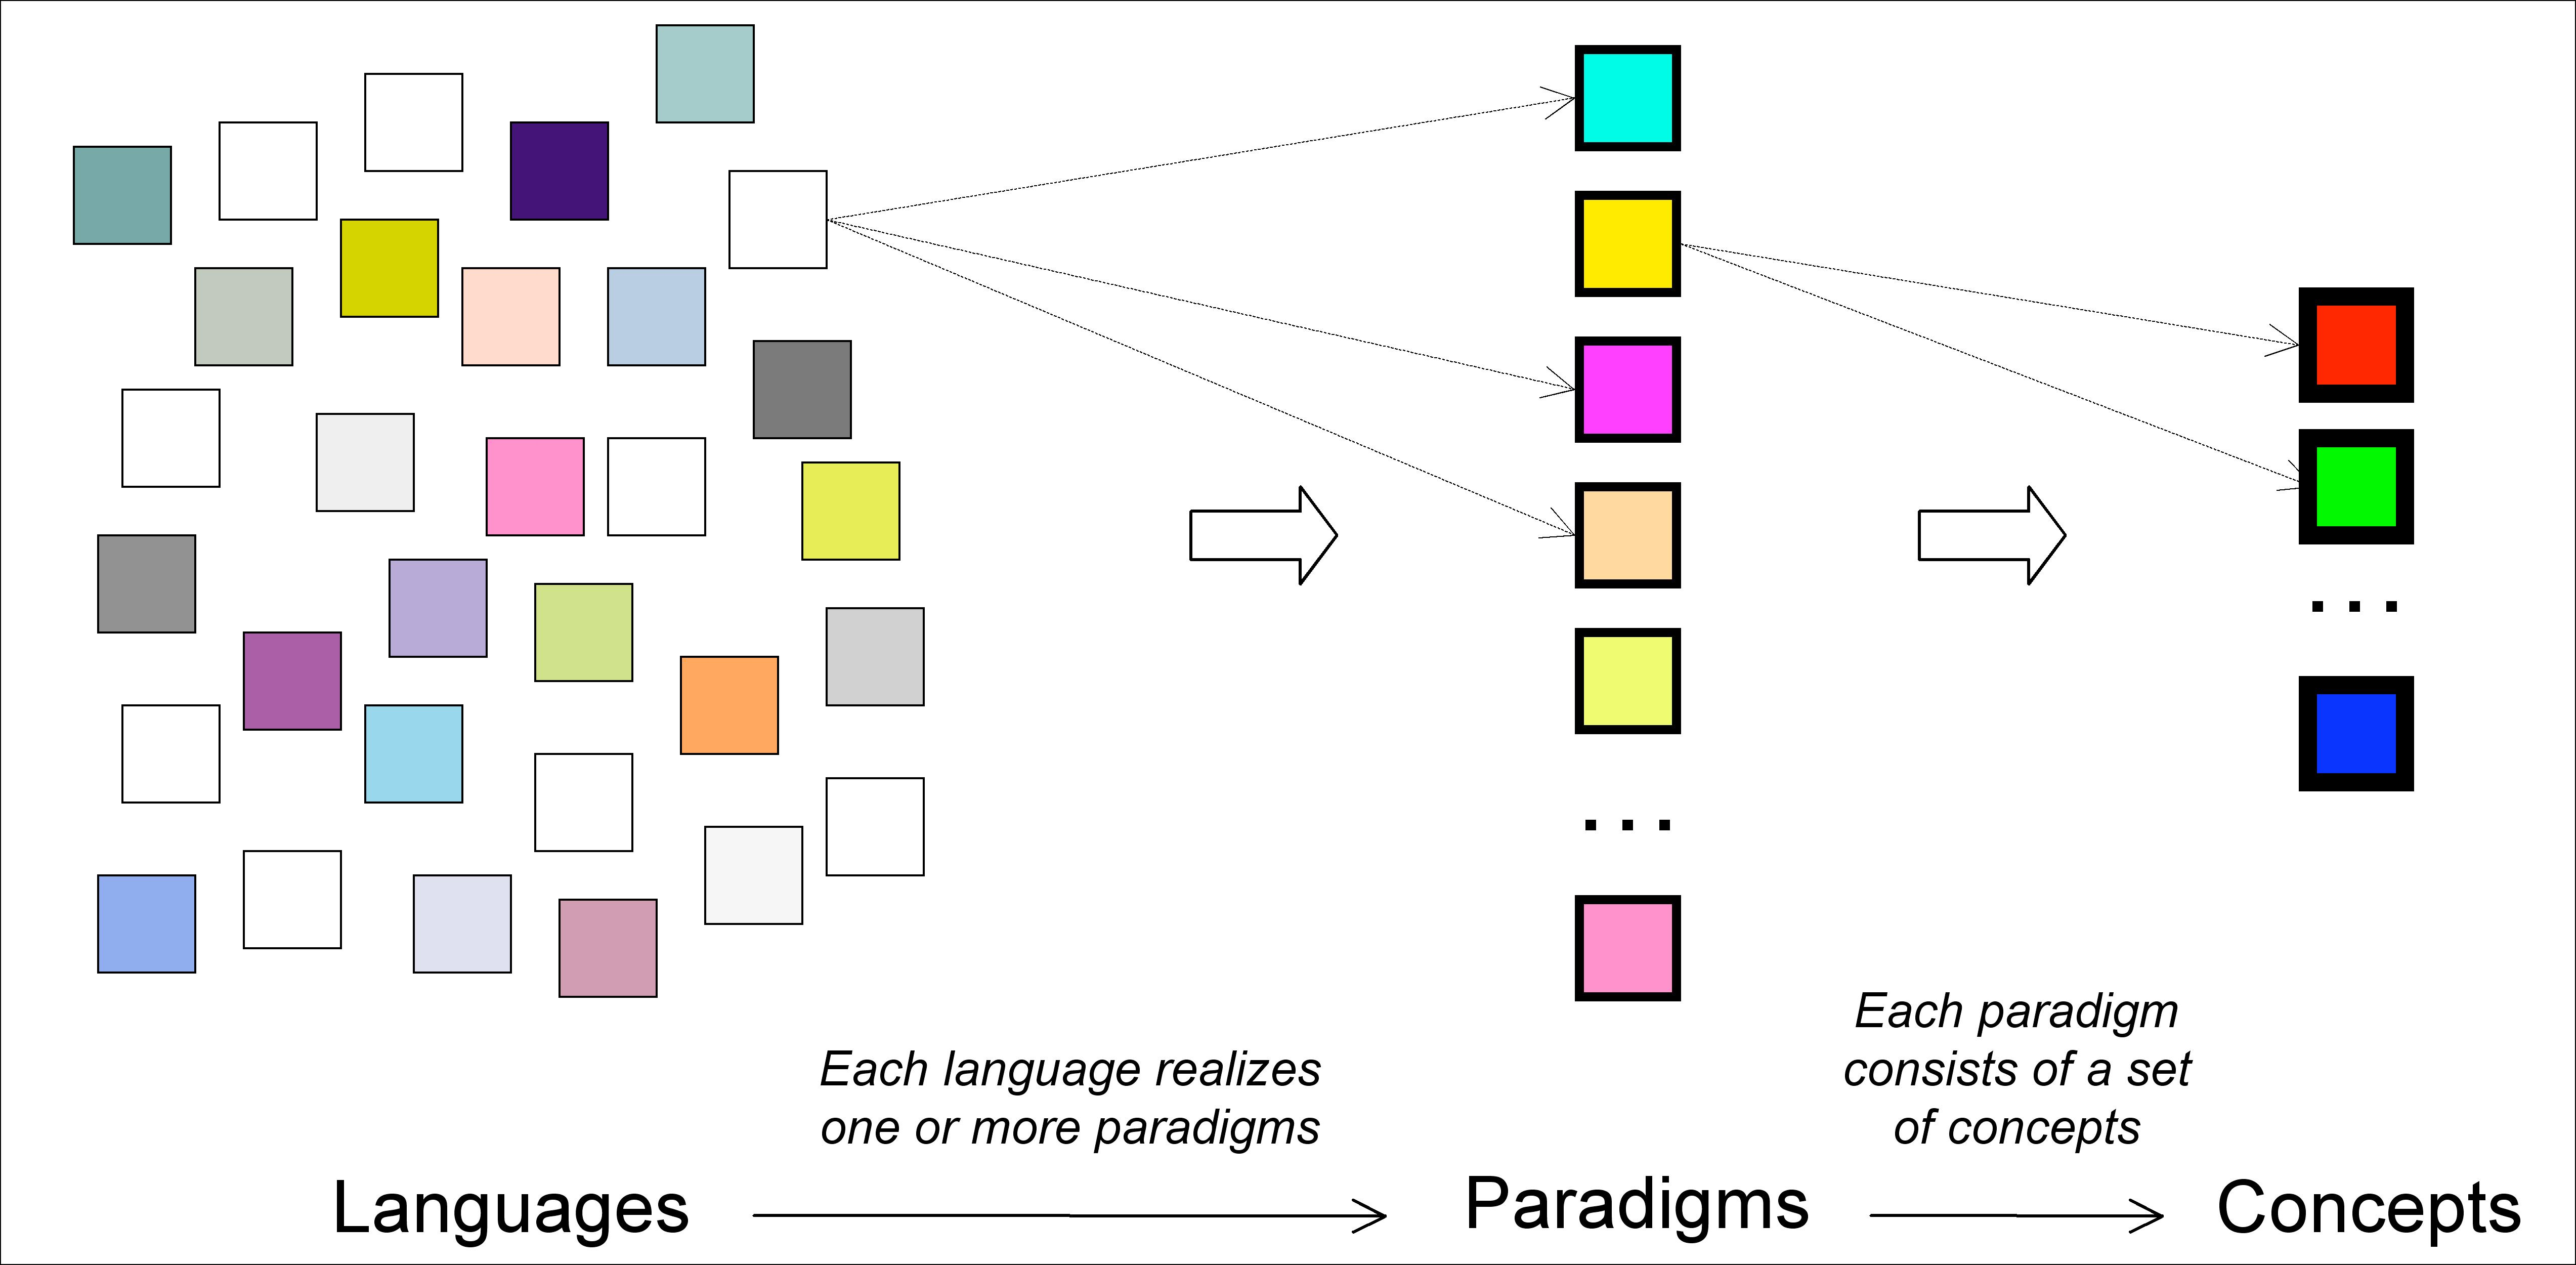
\includegraphics[width=12cm]{./fig/roy2009_languages_paradigms_and_concepts.jpeg}

  \small Fonte: \textcite[p.~12]{roy2009}.
  \label{img:LangsParadigmsConcepts}
\end{figure}

Da mesma forma que em engenharia de software (como um processo) pode-se adotar
diferentes metodologias de desenvolvimento, em linguagens de programação (como
modelos de computação) é desejável utilizar diferentes paradigmas de
programação.
Linguagens tradicionais como Java e C++ dão suporte a um ou dois paradigmas
diferentes.
“Isso é lamentável, pois problemas de programação diferentes precisam de
conceitos diferentes de programação para serem resolvidos claramente.”
\cite[p. 10]{roy2009}.

\textcite{roy2009} defende o uso de um modelo de programação \emph{multiparadigma},
porque:

\begin{citacao}
  Idealmente, uma linguagem deveria dar suporte a vários conceitos de forma
  bem integrada, para que o programador possa escolher os conceitos certos
  sempre que forem necessários, sem que um complique o outro.
  (p.~10; tradução nossa)
\end{citacao}

Apesar de linguagens tradicionais não dar suporte a esse modelo, entender os
conceitos certos pode melhorar a forma de programação, mesmo em linguagens que
não dê suporte direto a eles, assim como programação orientada a objetos é
possível em C com a atitude adequada \cite{roy2009}.

\textcite{roy2009} apresenta quatro modelos importantes que simplificam
programação concorrente em relação à linguagens convencionais: \emph{concorrência
declarativa}, \emph{programação funcional reativa}, \emph{programação síncrona
discreta}, e \emph{programação com restrições}.

No modelo declarativo de concorrência o resultado de um programa pode ser
calculado incrementalmente.
“Se a entrada de um programa concorrente é dada incrementalmente, então o
programa também irá calcular o resultado de saída incrementalmente.”
\cite[p. 238; tradução nossa]{roy2004}.
Esses paradigmas não possuem condições de corrida, \emph{‘race conditions’} em
inglês.
\todo{Esses últimos dois parágrafos parecem estar deslocados.}

\section{Programação Funcional}
\label{sec:org75febf5}
Programação Funcional (PF) é assim chamada porque sua operação básica é a
aplicação de funções à argumentos \cite{hughes1990}.
Lisp foi a primeira linguagem de programação funcional.
Criada em 1958 originalmente como uma notação matemática para programas de
computador, influenciada pelo \emph{cálculo lambda} de Alonzo Church.

Na matemática a ideia de \emph{quadrado de um número} pode ser expressa
algebricamente como uma função \(f(x)=x*x\).
Em Elm, \todo{Migrar os exemplos pra JavaScript.} a ideia de quadrado pode ser
expressa como \mintinline{elm}{quadrado x = x * x}.
A expressão pode ser lida em português da seguinte forma: “O quadrado de algo
é ele multiplicado por ele mesmo.”

A expressão algébrica denota uma função \(f\) que relaciona um número \(x\) com
seu quadrado, ou transforma \(x\) em seu quadrado.
A expressão em Elm define uma função \mintinline{elm}{quadrado} que transforma o
parâmetro \mintinline{elm}{x} em seu quadrado.
\textcite{roy2009} descreve uma função no contexto da PF:

\begin{citacao}
  Funções são funcões matemáticas: quando chamadas com os mesmos argumentos,
  elas sempre dão os mesmos resultados. Funções não mudam. No mundo real,
  as coisas são diferentes. Há poucas entidades reais que têm o comportamento
  intemporal das funções. Organismos crescem e aprendem. Quando o mesmo
  estímulo é dado à um organismo em momentos diferentes, a reação geralmente
  será diferente. (p. 26; tradução nossa)
\end{citacao}

Um programa funcional é uma expressão a ser avaliada, no contexto de um
conjunto de definições — principalmente definições de funções.
Por exemplo, dada as definições de função em \ref{code:programfnDefinitions}, um
programa pode consistir da expressão \mintinline{elm}{dobrar (somar 2 3)} e o resultado
do programa então seria \mintinline{elm}{10} \cite{noble1994}.

\begin{listing}[H]
  \centering
  \caption{Definição das funções \texttt{somar} e \texttt{dobrar}.}
  \begin{minted}[linenos=false]{elm}
    somar x y = x + y
    dobrar z = 2 * z
  \end{minted}
  \small Fonte: Adaptado de \textcite{noble1994}.
  \label{code:programfnDefinitions}
\end{listing}

Funções são consideradas \emph{cidadãs de primeira classe — do inglês ‘first-class
citizens’}, e podem ser passadas como argumentos da mesma forma que qualquer
outro tipo de dado.
Uma função é definida para ter um certo número de argumentos (sua \emph{aridade}),
mas se for calculada com menos argumentos o resultado é outra função.
Isso permite funções como as definidas em \ref{code:currying}, onde \texttt{inc} recebe
um número e adiciona \texttt{1} a ele, e \texttt{tres} aplica \texttt{f}, uma dada função, três
vezes à qualquer argumento em que \texttt{f} normalmente aceitaria, por exemplo: a
expressão \texttt{tres inc 2} resulta no valor \texttt{5} \cite{noble1994}.

\begin{listing}[H]
  \centering \caption{\emph{Currying}.}
  \begin{minted}[linenos=false]{elm}
    inc = somar 1
    tres f = f >> f >> f >>
  \end{minted}
  \small Fonte: Adaptado de \textcite{noble1994}.
  \label{code:currying}
\end{listing}

\section{Programação Reativa}
\label{sec:orgb0b9adc}
Programação reativa abrange um leque enorme de conceitos de programação.
Isso se deve pela escolha da palavra ‘reativa’, que diz mais sobre uma
\emph{propriedade do que se programa} do que sobre um \emph{conceito de programação}.
Vários conceitos e paradigmas diferentes podem ser empregados na programação
de uma aplicação reativa — ou de qualquer tipo de programa \cite{roy2009}.
Entende-se então o porquê do paradigma abarcar tantos conceitos.
Portanto, faz sentido descrever \emph{programas reativos} e a propriedade
\emph{reativa}, antes de discutir os modelos de programação disponíveis para
abordá-los.
A \emph{priori}, é conveniente distinguir entre três tipos de programas de
computador:

\begin{itemize}
\item \emph{programa transacional}: computa resultados a partir de um dados conjunto de
dados de entrada. Compiladores e programas de computação numérica são alguns
exemplos clássicos;
\item \emph{programa interativo}: interage, no seu próprio ritmo, com usuários ou com
outros programas. Sistemas de tempo compartilhado são interativos, do ponto
de vista do usuário;
\item \emph{programa reativo}: também mantém interação contínua com seu ambiente, mas
no ritmo determinado pelo ambiente, não pelo próprio programa. Interfaces
gráficas\footnote{Este tipo de programa é popularmente conhecido como interativo — nota-se muito o
uso da expressão ‘Aplicações interativas’ por exemplo.} e robôs são alguns exemplos muito comuns.
\end{itemize}

Programas interativos computam no seu próprio ritmo e tratam, em grande parte,
de comunicação.
Enquanto programas reativos só computam em resposta a demanda externa e lidam
principalmente com eventos ou interrupções de hardware \cite{berry1989}.
\emph{Interfaces gráficas} reagem a cliques do mouse, pressionamento de teclas,
gestos multitoque, etc.
\emph{Sistemas embarcados} reagem a sinais de hardware.
E \emph{programas de monitoração e controle} reagem a mudanças no ambiente externo
\cite{salvaneschi2015}.

Programação reativa é um paradigma que dá suporte à programação de aplicações
reativas através de alguns conceitos específicos.
Alguns deles são:

\begin{itemize}
\item \emph{fluxos de eventos\footnote{Tradução literal de \emph{‘event streams’}, em inglês.}}: servem para modelar notificações
discretas;
\item \emph{propagação automática de alterações}: o modelo de execução automaticamente
repercuti alterações nos dados;
\end{itemize}

PR é compartilha muitos conceitos com o paradigma de \emph{Programação Funcional
Reativa (PFR)}.
Os dois geralmente são confundidos na comunidade de praticantes.
PFR possui dois conceitos importantes que o diferencia da PR.
O primeiro é o conceito de \emph{tempo contínuo} — na PR o tempo é discreto.
O segundo é o conceito de \emph{semântica denotacional}.
PFR é mais indicada para domínios que precisam representar tempo contínuo,
como simulações físicas.
PR é mais indicada para sistemas reativos, como é explicado por
\textcite{roy2009}:

\begin{citacao}
  Usar tempo discreto simplifica enormemente a programação de sistemas reativos.
  Por exemplo, isso significa que subprogramas podem ser compostos de forma
  trivial: os eventos de saída de um subcomponente estão instantaneamente
  disponíveis como eventos de entrada para outros subcomponentes.
  (pg. 36; tradução nossa)
\end{citacao}
